\documentclass[12pt]{report}
\usepackage{graphicx}
\usepackage{amsmath}
\usepackage{fancyhdr}
\usepackage{geometry}
\usepackage{circuitikz}
\usepackage{subfigure}
\usepackage{caption}
\usepackage{karnaugh-map}

\geometry{letterpaper, margin=1in}
\graphicspath{{./images/}}

% Header and Footer
\pagestyle{fancy}
\fancyhf{}
\fancyhead[L]{CSE 2301 - Lab 03: I/O and POSTNET}
\fancyhead[R]{\thepage}
\setlength{\headheight}{15pt}

\author{Arturo Salinas-Aguayo}
\title{Lab 03: I/O and POSTNET3: I/O and POSTNET3: I/O and POSTNET}
% theorem set
\newtheorem{example}{Example}
% Example block environment
\newenvironment{examp}
{\vspace{0.5cm}
\hrule
\begin{example}}
{\hrule
\vspace{0.5cm}
\end{example}}

\begin{document}
\newcommand{\closure}[2][3]{%
	{}\mkern#1mu\overline{\mkern-#1mu#2}}
\newcommand\ncoverline[1]{\mkern1mu\overline{\mkern-1mu#1\mkern-1mu}\mkern1mu}
% Title Page
\begin{titlepage}
	\centering
	\vspace*{3cm}
	\huge\textbf{Lab 03: I/O and POSTNET}\\
	\vspace{5cm}
	\Large\textbf{Arturo Salinas-Aguayo}\\
	\normalsize
	CSE 2301: Principles and Practice of Digital Logic Design\\
	Dr. Mohammad Khan, Section 003L-1248\\
	Electrical and Computer Engineering Department
	\vfill
	
\includegraphics[scale=0.1]{uconnlogo}\\
	College of Engineering, University of Connecticut\\
	\scriptsize{Coded in \LaTeX}
	\vspace*{1cm}
\end{titlepage}
\section*{Theory}
\subsection*{The 7405 Chip DIP}
The \textbf{7405 DIP} \textit{(Dual-Inline-Package)} from Texas Instruments is a different kind of inverter called an \textit{Open Collector}, compared to the \textbf{7404 DIP} by the same manufacturer which is a standard inverter with something called a \textit{Push-Pull Output Stage.} Our application requires driving a load, in this case some Light Emitting Diodes. These LEDs require higher current draw which a \textbf{7404} IC cannot handle directly. The \textbf{7405} provides the ability to drive an external load by pulling the output signal to ground without having to supply or drive the current from the IC itself.

\subsubsection*{The Bipolar Junction Transistor}
In order to properly explain this choice, the \textit{emitter, base,} and \textit{collector} of a Bipolar Junction Transistor must be properly defined.
\begin{examp}
	\textbf{The Bipolar Junction Transistor Abstraction}
	\newline
	\textbf{Emitter}
	\textnormal{A \textit{heavily} doped, medium-sized layer designated to inject or emit electrons.}
	\newline
	\textbf{Base}
	\textnormal{A thin layer of \textit{medium} doped material designed for electron transmission.}
	\newline
	\textbf{Collector}
	\textnormal{A wide layer of \textit{lightly} doped material designed to \textit{collect} electrons.}
	\newline
	Texas Instruments utilizes NPN Transistors in their schematics such as this:
	\begin{figure}[h]
		\center{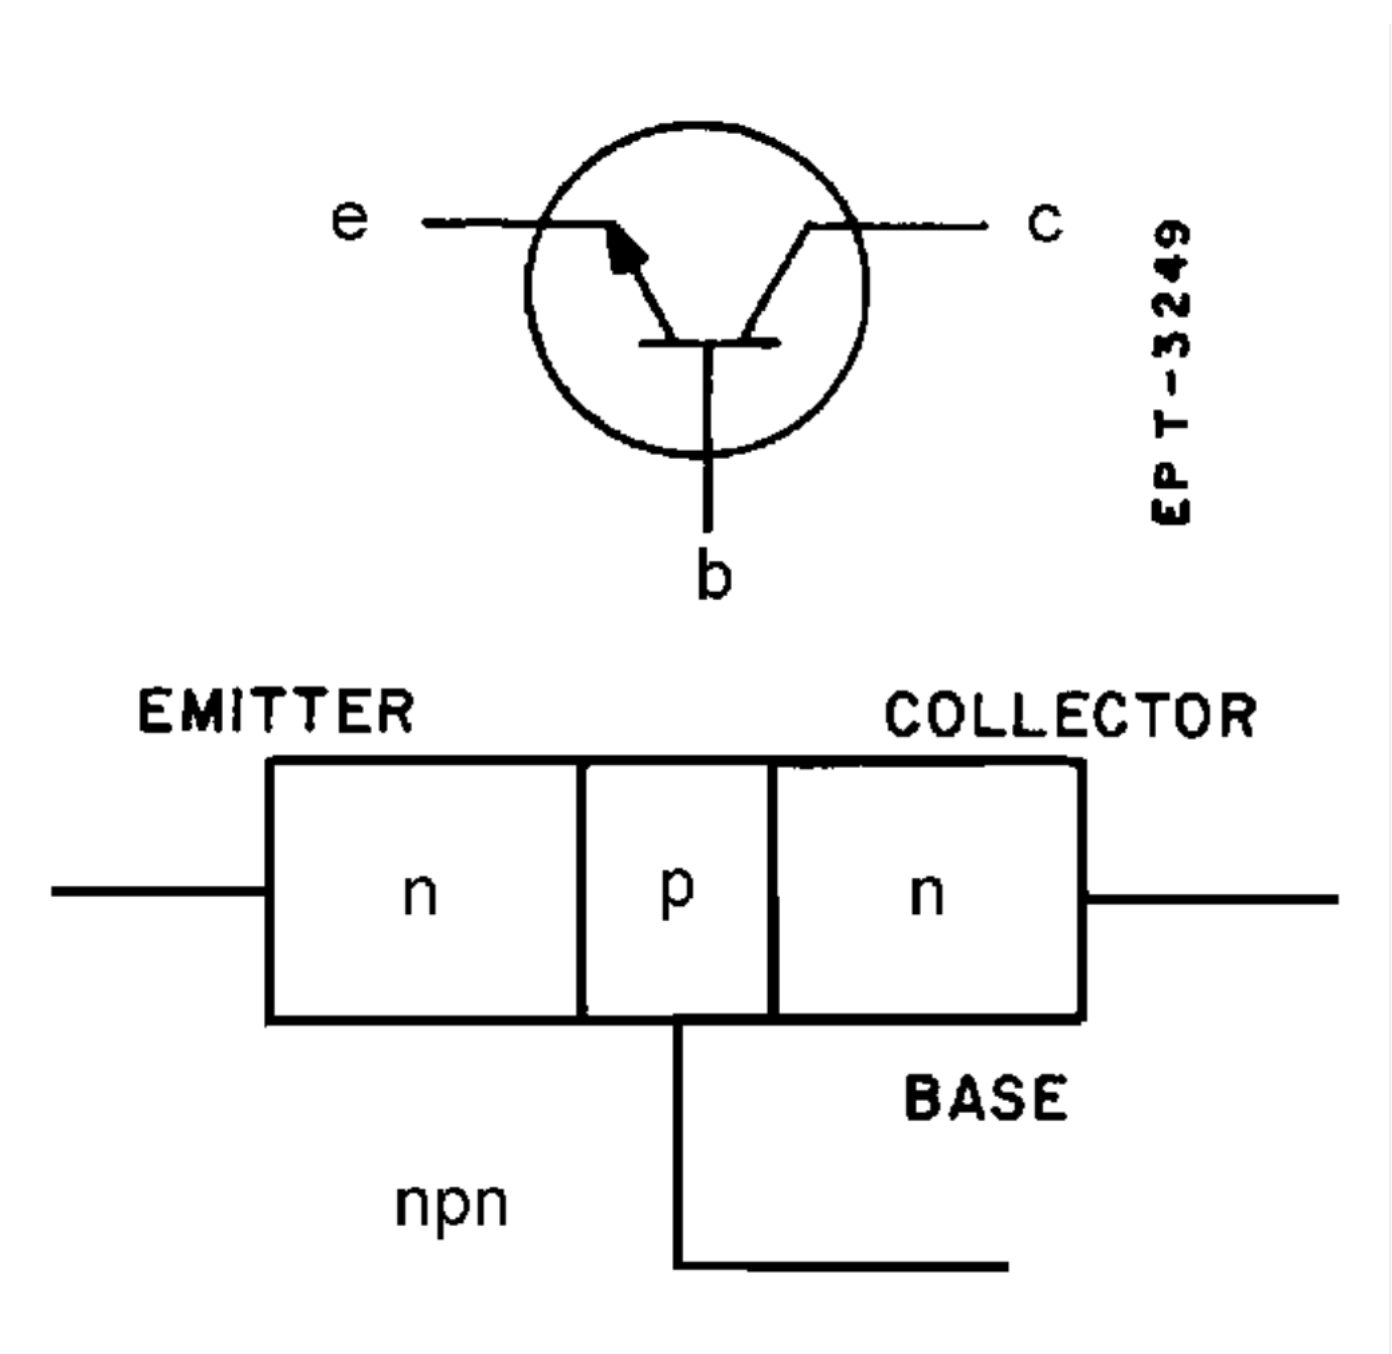
\includegraphics[scale=0.3]{NPN}}
		\captionof{figure}{The NPN Transistor}
	\end{figure}
\end{examp}
\subsubsection*{Why the 7405?}
All of this hand waving still doesn't answer the question as the difference hasn't been hammered home quite yet.

\textbf{Example 2} shows the schematics from the official Texas Instrument's Datasheets and walks through the operation. When focusing on the output \(Y\), the difference between the circuits is clear.
The 7405 chip's output BJT's collector terminal is left unconnected within the chip. This is also known as an ``open." This architecture allows the chip to be independent of the downstream current draw.

This makes it suitable for applications where a resistive load such as a motor, or in this case, an LED is connected to the output of the inverter.
This does require some planning as the load requires a external pullup resistor in order to achieve a HIGH output.

There are three possible different configurations of a BJT circuit, a common emitter, common base, or a \textit{common collector circuit} where ``Common" references which two leads of the BJT are both part of the input and outputs circuits.

For the 7405, a positive-going input signal drives the base more positive with respect to the emitter, which causes the base current to increase. This results in more emitter current, causing a more positive output voltage at the emitter to drive our LED.
\begin{examp}
	\textbf{Operation of the 7405}
	\begin{figure}[h]
		\subfigure[The Standard 7404]{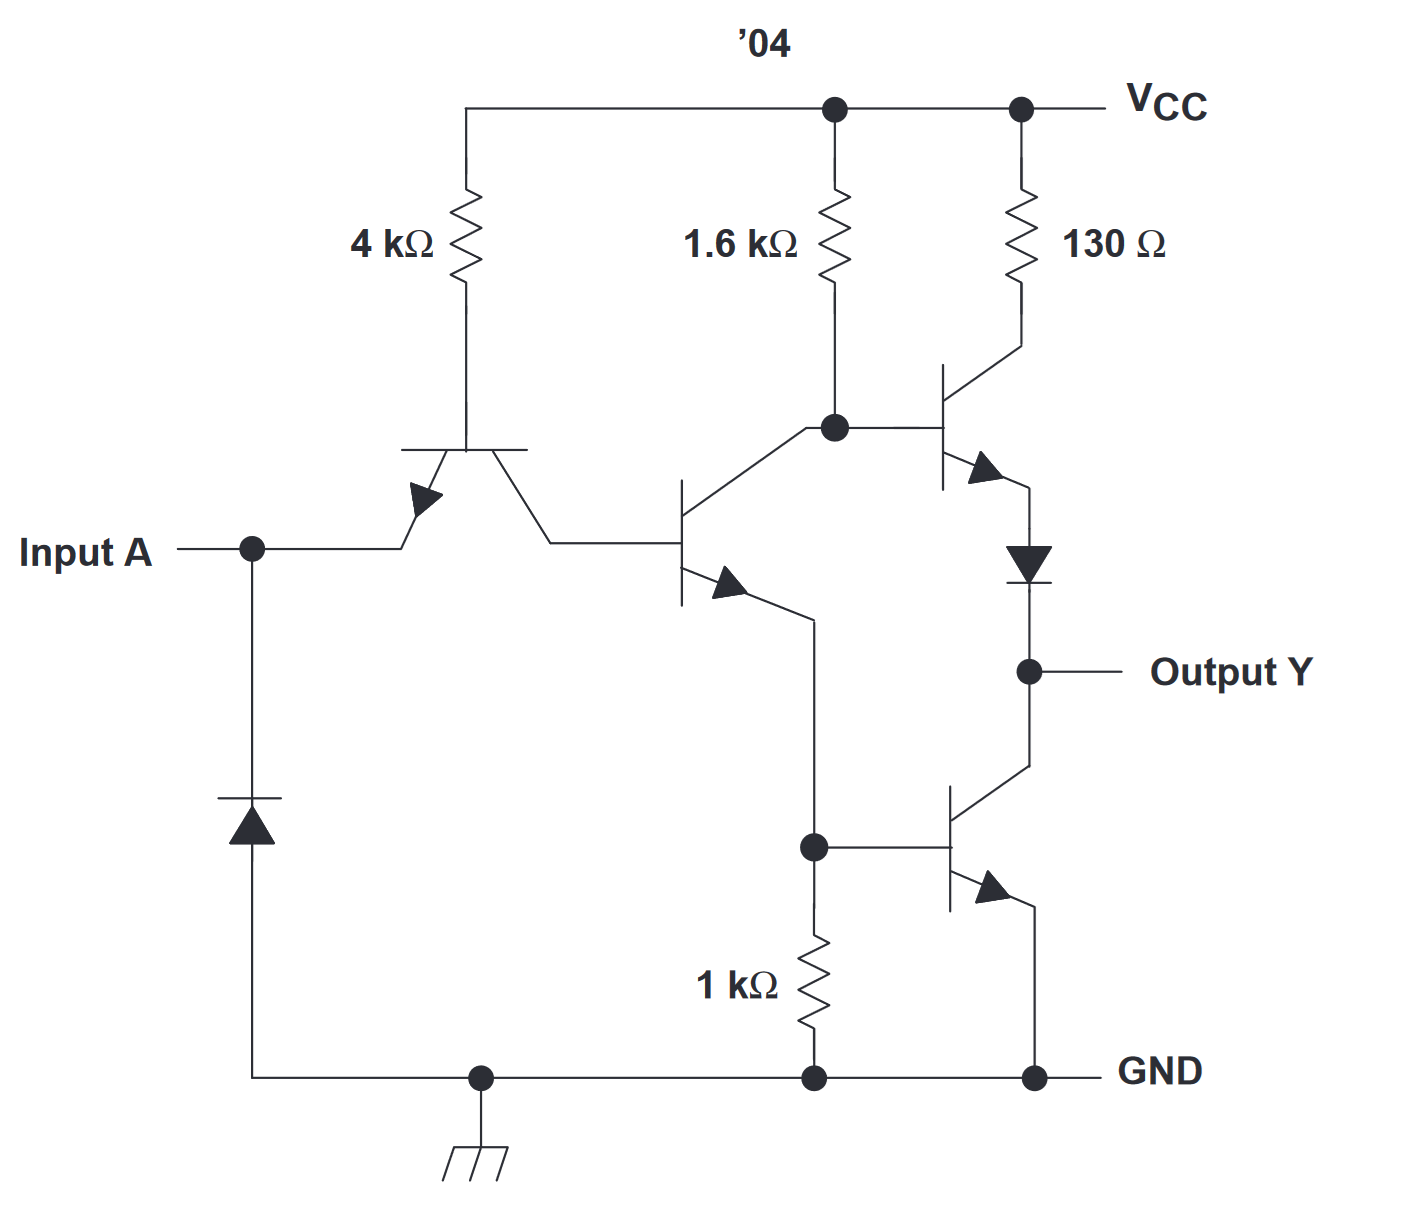
\includegraphics[width=8cm]{04}}
		\hfill
		\subfigure[The Standard 7405]{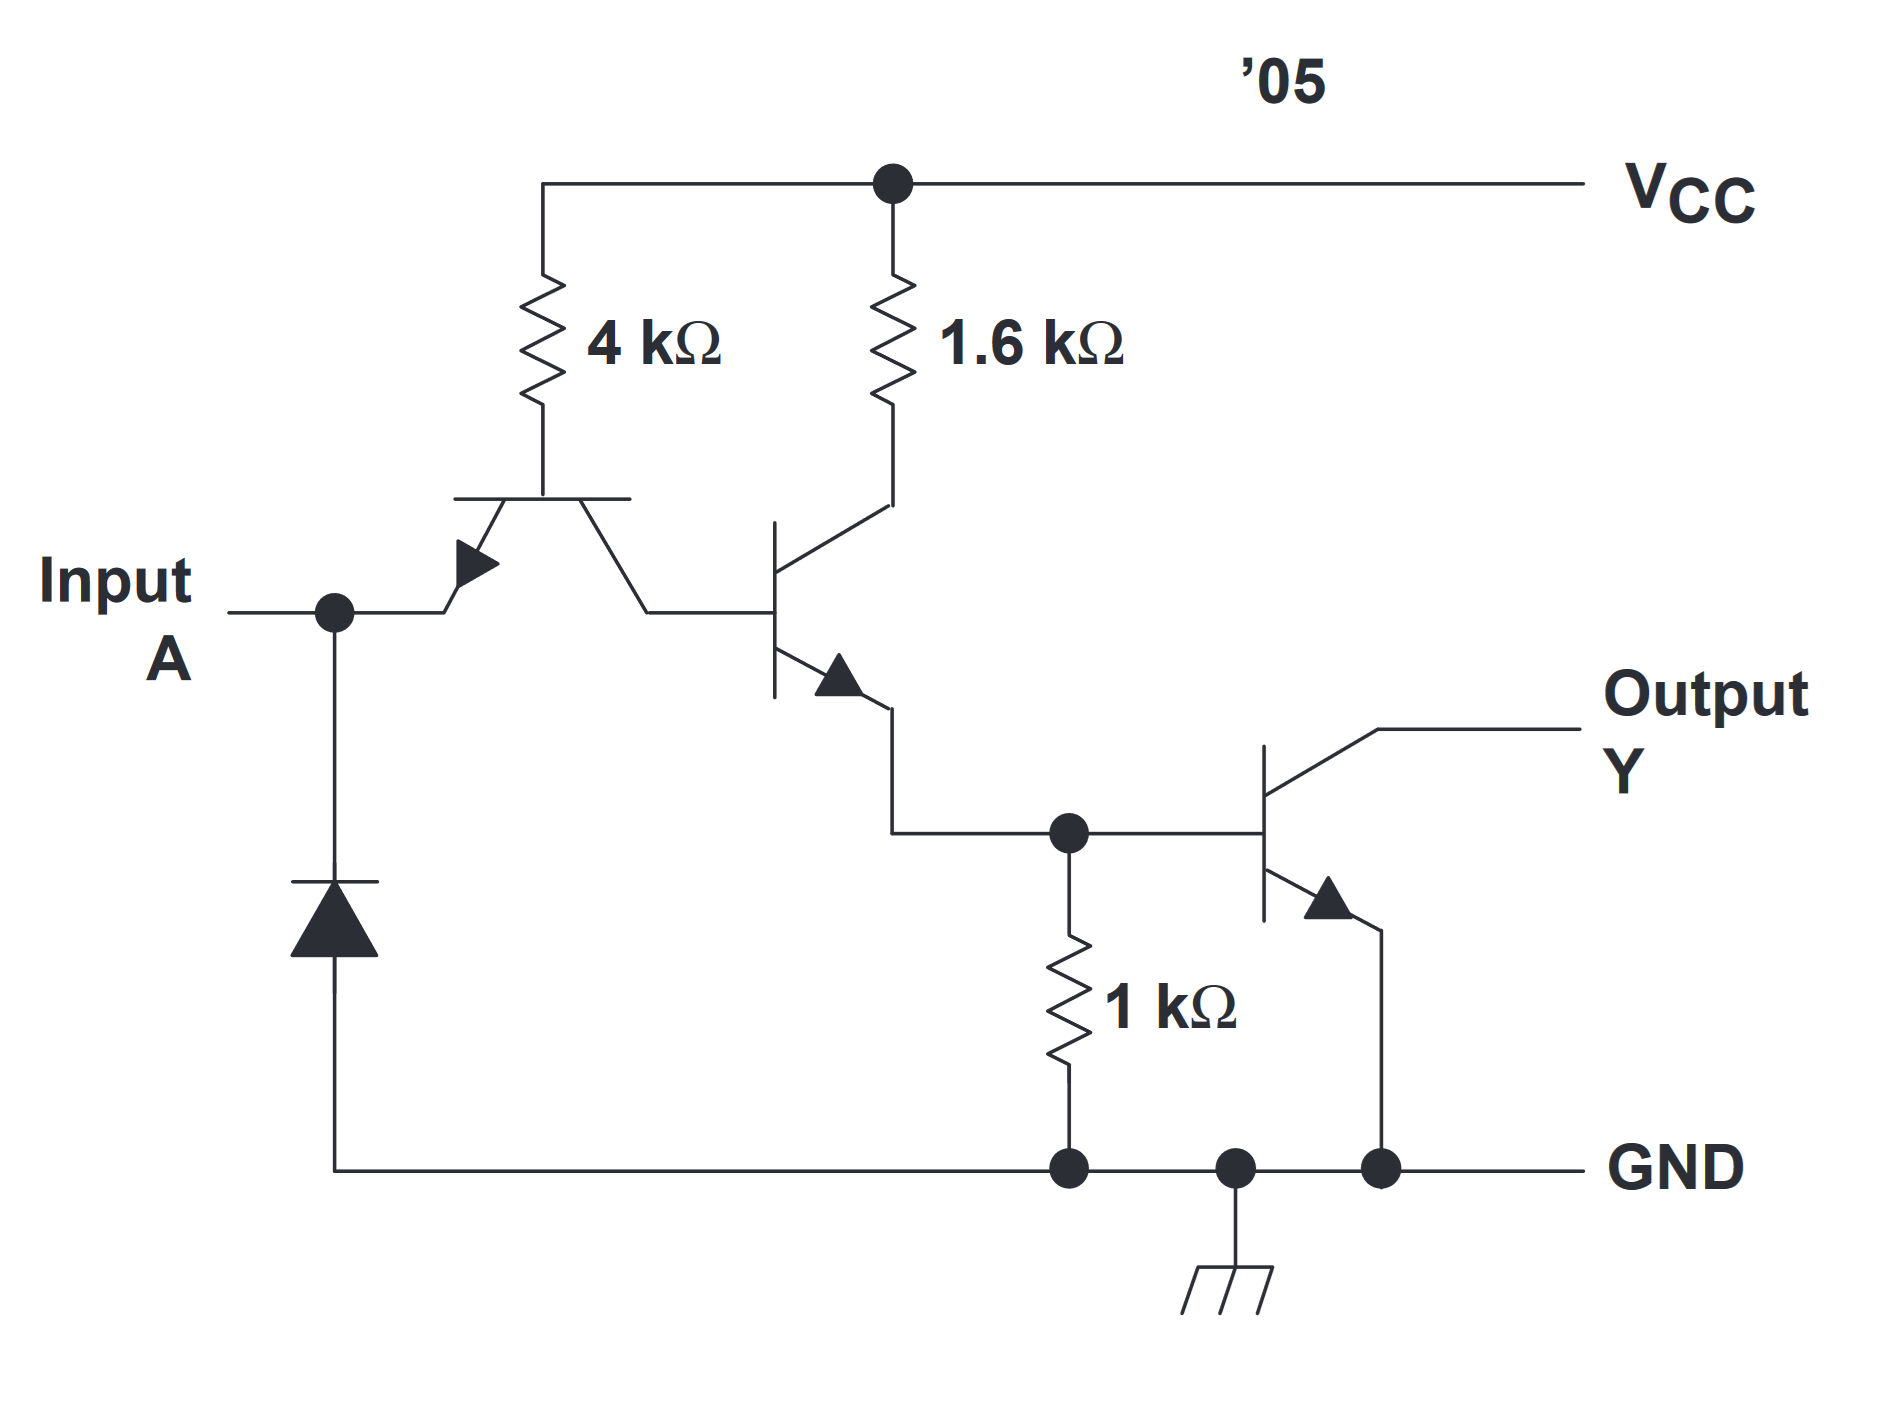
\includegraphics[width=8cm]{05}}
		\captionof{figure}{Schematic View}
	\end{figure}
	\newline
	\textnormal{When the input signal is high:}
	\begin{itemize}

		\item The base of the first NPN transistor is forward biased relative to its emitter, allowing base current to flow. This results in current flowing from the collector to the emitter, effectively grounding the output.
		\item The base current enables a larger current flow from the collector to the emitter, pulling the output low (close to ground).
		\item In this state, the transistor is ``on," and the output is a logic LOW signal (approximately 0.0V to 0.8V in TTL logic).
	\end{itemize}
	\pagebreak
	\textnormal{When the input signal is low:}
	\begin{itemize}
		\item The base of the first NPN transistor is not forward biased, so no current flows through the base-emitter junction. As a result, the collector-emitter path remains open, and the transistor is turned off.
		\item Since the transistor is off, the output floats and is pulled high by the external pull-up resistor, resulting in a logic HIGH output close to \(V_{CC}\).
	\end{itemize}
\end{examp}
In the 7405 open-collector configuration, the NPN transistor plays a crucial role in determining the output state based on the input signal.

As with any NPN transistor, the emitter, base, and collector function to control the current flow between the collector and emitter through the base current.

In this circuit, the NPN transistor's collector is left unconnected internally (hence the term ``open collector"). The external load, such as an LED or a resistive element, is connected between the output (collector) and a pull-up resistor, which is tied to the supply voltage

In essence, the NPN transistor in the 7405 circuit acts as a switch that controls the flow of current to the output based on the base current. When there is base current, the transistor conducts, and the output is pulled low. When there is no base current, the transistor is off, and the output is pulled high by the external resistor.

This open-collector design is particularly useful for applications that require the driving of higher-current loads, such as LEDs, without requiring the IC itself to supply the current. Instead, the external load provides the necessary current, allowing the circuit to handle higher loads more efficiently.

To summarize, in plain non-electrical engineering speak, if the transistor is ON, current flows through the path of least resistance and robs the output (our LED) of its current, making the light go dim. If the transistor is OFF, the pullup resistor now makes the path of least resistance between the LED and ground and the LED illuminates.
\subsection*{Current Draw of Each LED} \
The current through each LED is calculated using Ohm's Law:
\begin{examp}
	\[
		I = \frac{V_{R}}{R} = \frac{V_{\text{supply}} - V_{\text{LED}}}{R}
	\]

	Where:
	\begin{itemize}
		\item \( V_{\text{supply}} = 5V \) is the supply voltage.
		\item \( V_{\text{LED}} \) is the forward voltage of the LED.
		      This is measured at \(1.786V\) by my multimeter.
		\item \( R = 330 \, \Omega \) is the resistor value.
	\end{itemize}
	\[
		I_{\text{red}} = \frac{5V - 1.786V}{330 \, \Omega} = \frac{3.214V}{330 \, \Omega} = 9.74 \, \text{mA}
	\]
\end{examp}
\pagebreak
\subsection*{POSTNET to $XS_{3}$ Encoding}
\begin{table}[h!]
	\centering
	\begin{tabular}{|c|c c c c c|c c c c|}
		\hline
		Decimal & V & W & X & Y & Z & D & C & B & A \\
		\hline
		0       & 1 & 1 & 0 & 0 & 0 & 0 & 0 & 1 & 1 \\
		1       & 0 & 0 & 0 & 1 & 1 & 0 & 1 & 0 & 0 \\
		2       & 0 & 0 & 1 & 0 & 1 & 0 & 1 & 0 & 1 \\
		3       & 0 & 0 & 1 & 1 & 0 & 0 & 1 & 1 & 0 \\
		4       & 0 & 1 & 0 & 0 & 1 & 0 & 1 & 1 & 1 \\
		5       & 0 & 1 & 0 & 1 & 0 & 1 & 0 & 0 & 0 \\
		6       & 0 & 1 & 1 & 0 & 0 & 1 & 0 & 0 & 1 \\
		7       & 1 & 0 & 0 & 0 & 1 & 1 & 0 & 1 & 0 \\
		8       & 1 & 0 & 0 & 1 & 0 & 1 & 0 & 1 & 1 \\
		9       & 1 & 0 & 1 & 0 & 0 & 1 & 1 & 0 & 0 \\
		\hline
	\end{tabular}
	\caption{POSTNET to XS3 Conversion Table}
\end{table}

\begin{examp}
\textbf{D Output}

The map is divided into two layers for $V=0$ and $V=1$. Pay Attention to $V$.
\begin{center}
\begin{karnaugh-map}(label=corner)[4][4][2][$Z$][$Y$][$X$][$W$][$V$]
\minterms{10,12,26,28}
\maxterms{3,5,6,8,19,21,22,25}
\autoterms[X]
\implicant{12}{14}[0]
\implicant{15}{10}[0]
\implicant{0}{6}[1]
\end{karnaugh-map}
\end{center}

This produces:
\[
	D = V(\closure{W}) + \closure{V}(WX + WY)
\]
\[
	D = V\closure{W} + \closure{V}WX + \closure{V}WY \quad \text{(Distribution)}
\]
\[
	D = V\closure{W} + WX + WY \quad \text{(Absorption)}
\]
\end{examp}
\newpage
\begin{examp}
\textbf{C Output}
\begin{center}
\begin{karnaugh-map}(label=corner)[4][4][2][$Z$][$Y$][$X$][$W$][$V$]
\minterms{4,19,21,22,25}
\maxterms{1,2,8,28,26}
\autoterms[X]
\implicant{4}{14}[0]
\implicantedge{0}{1}{8}{9}[1]
\implicant{0}{6}[1]
\end{karnaugh-map}
\end{center}

This produces:
\[
	C = \closure{V}(\closure{W} + \closure{X}Y) + V(X)
\]
\[
	C = \closure{V}\closure{W} + \closure{V}\closure{X}Y + VX \quad \text{(Distribution)}
\]
\end{examp}

\begin{examp}
\textbf{B Output}
\begin{center}
\begin{karnaugh-map}(label=corner)[4][4][2][$Z$][$Y$][$X$][$W$][$V$]
\minterms{6,9,17,18,20,24}
\maxterms{3,5,12,10}
\autoterms[X]
\implicant{0}{10}[1]
\implicantedge{0}{1}{8}{9}[0]
\implicant{7}{14}[0]
\end{karnaugh-map}
\end{center}

This produces:
\[
	B = V + \closure{V}(W\closure{Y} + XY)
\]
\[
	B = V + \closure{V}W\closure{Y} + \closure{V}XY \quad \text{(Distribution)}
\]
\end{examp}
\newpage
\begin{examp}
\textbf{A Output}
\begin{center}
\begin{karnaugh-map}(label=corner)[4][4][2][$Z$][$Y$][$X$][$W$][$V$]
\minterms{5,12,9,18,20,24}
\maxterms{17,3,6,10}
\autoterms[X]
\implicant{0}{9}[0]
\implicantedge{0}{4}{2}{6}[1]
\implicant{12}{10}[1]
\end{karnaugh-map}
\end{center}
This produces:
\[
	A = \closure{V}\closure{Y} + V(\closure{W}\closure{Z} + \closure{W})
\]
\[
	A = \closure{V}\closure{Y} + V\closure{W}\closure{Z} + V\closure{W} \quad \text{(Distribution)}
\]
\end{examp}
\newpage
\[ E = r \cdot \log_r N \]
where $E$ is the economy, $r$ is the radix (base) of the number system, and $N$ is the number of unique values to be represented. \

This metric balances two competing factors:
\begin{itemize}
	\item The number of unique digits required (complexity)
	\item The number of digit positions needed to represent a given range of values (length)
\end{itemize}

A lower value of $E$ indicates a more economical system, offering a better trade-off between these factors.

\subsubsection*{Implications and Applications}
Systems with good radix economy can offer several advantages:
\begin{itemize}
	\item Enhanced human readability
	\item Reduced system complexity
	\item More compact and efficient computational implementations
	\item Potential for reduced physical space requirements in hardware
	\item Improved circuit performance and reduced power consumption
	\item Potential for lower overall project costs in hardware design
\end{itemize}
\subsubsection*{Optimal Radix vs. Practical Considerations}

Mathematically, the optimal radix for maximal economy is $e \approx 2.718$ which is derived by using the second derivative test to determine the maximum value. However, practical considerations often outweigh pure mathematical optimality

Binary (\textit{radix-2}) systems are prevalent in computing despite not having the best radix economy. The simplicity of binary representation, with only two states (0 and 1), greatly simplifies computer architecture and logic design. This simplicity often outweighs the theoretical advantages of more economical bases in real-world applications.

The choice of number system thus involves a balance between theoretical efficiency and practical implementation constraints.

% Deliverables Section
\section*{Deliverables}
After calculating the minterms for our \(Z_{0}, Z_{1}, Z_{2}, Z_{3}\) outputs, that is, the equations such that our corresponding output bit is TRUE (1), we get some fairly large equations that were then able to get reduced by boolean logic algebra. Unfortunately, because the lab limited us to only two-input OR, AND, and one-input NOT gates, the simplicity of the circuit was not able to get greatly reduced.
\begin{examp}
	Outputs \( Z_3, Z_2, Z_1, Z_0 \):
	\begin{itemize}
		\item \( Z_0 = \closure{D}\closure{C}\closure{B}A + \overline{D}C\overline{B}\closure{A} + \overline{D}CBA + D\overline{C}B\overline{A} \) \\
		      \( Z_0 = \closure{D}\closure{C}BA + C{B A} + CBA) + D\overline{C}B\overline{A} \) \\
		      \( Z_0 = \overline{D}(\closure{C}\closure{B}A + C(\closure{B}\closure{A}\ + BA)) + D\overline{C}B\overline{A} \) \\
		      The \( Z_0 \) bit could be simplified by grouping the \( \overline{D} \) signal to the outside of common multiples and some mild reduction utilizing distributivity and identity boolean algebra rules.
		\item \( Z_1 = \closure{D}\closure{C}B\overline{A} + \overline{D}C\overline{B}A + D\closure{C}\closure{B}\closure{A}\) \\
		      \( Z_1 = \overline{D}(\overline{C}B\overline{A} + C\overline{B}A) + D\closure{C}\closure{B}\closure{A}\) \\
		      The \( Z_1 \) bit could also be simplified by grouping the \( \overline{D} \) signal to the outside of common multiples. \

		\item \( Z_2 = 0 \quad \text{(Always FALSE)} \)

		\item \( Z_3 = 0 \quad \text{(Always FALSE)} \)
	\end{itemize}
\end{examp}
% Discussion Section
% TODO: Discussion needs to be expanded
\section*{Discussion}
The practical portion of the lab was more involved with Logicworks as we learned about simplifying Boolean expressions. The inclusion of the Hex Keyboard into the schematic allowed for a nicer way of interacting with the circuits and careful wire routing throughout the workspace was crucial for success in completing this. Ultimately, the simplifications couldn't be applied as much as I initially thought that would be possible when it came to designing the circuit, but nevertheless each network of signals was easily troubleshot and ran through until the target output was reached.

Practically, this was quite engaging as the network of wires needed to be very closely monitored to ensure that a certain system wouldn't change after modification. After some troubleshooting and careful analysis of wire and inverter placement, the circuit was able to run, and the desired truth table was output successfully.

To conclude and summarize, the Lab reinforced concepts learned in class through pen and paper arithmetic and familiarity with the Digital Design Software tools in Logicworks.
% Practice Questions Section
\section*{Practice Questions}
\subsection*{Radix Conversion} \
Given the decimal number \(92_{10}\) we can change between number systems utilizing the algorithm discussed previously.
\begin{examp}
	\textbf{Binary:}
	\[
		92_{10} = (1 \cdot 2^6) + (0 \cdot 2^5) + (1 \cdot 2^4) + (1 \cdot 2^3) + (1 \cdot 2^2) + (0 \cdot 2^1) + (0 \cdot 2^0)
	\]
	\[
		92_{10} = 1011100_2
	\]
\end{examp}

\begin{examp}
	\textbf{Octal:}
	\[
		92_{10} = (1 \cdot 8^2) + (3 \cdot 8^1) + (4 \cdot 8^0)
	\]
	\[
		92_{10} = 134_8
	\]
\end{examp}

\begin{examp}
	\textbf{Hexadecimal:}
	\[
		92_{10} = (5 \cdot 16^1) + (12 \cdot 16^0) \quad \text{(where \(C = 12\))}
	\]
	\[
		92_{10} = 5C_{16}
	\]
\end{examp}
\pagebreak
\subsection*{2's Compliment and Decimal Conversion}
Given the signed binary number \(11001101_2\) swapping between 2's compliment and decimal is extremely easily. Begin by looking at the Most-Significant-Bit (MSB) for the first information about what decimal number this signed binary number contains. An MSB of 1 indicates a negative number, an MSB of 0 represents a positive number.

The two's complement representation facilitates simpler arithmetic operations and algorithms in digital systems. However, this comes at the cost of a reduced range for the maximum positive number that can be represented, compared to unsigned integers of the same bit length.
\begin{examp}
	\textbf{Size limits} \\
	Unsigned 8-bit integer:
	\begin{itemize}
		\item Range: $0 \to 2^8 - 1$ (0 to 255)
	\end{itemize}
	Signed 8-bit integer (two's complement):
	\begin{itemize}
		\item Positive range (MSB = 0): $0 \to 2^7 - 1$ (0 to 127)
		\item Negative range (MSB = 1): $-2^7 \to -1$ (-128 to -1)
	\end{itemize}
	\noindent\textbf{Note:} The signed range includes one more negative number (-128) than positive number (127) due to the nature of two's complement representation.
\end{examp}
\begin{examp}
	\textbf{Two's Complement Conversion:} \\
	Flip the bits and add 1.
	\[
		\begin{aligned}
			11001101_2  & \quad \text{(original number)}         \\
			00110010_2  & \quad \text{(flipped bits)}            \\
			+00000001_2 & \quad \text{(add 1)}                   \\
			\hline
			00110011_2  & \quad \text{(two's complement result)} \\
		\end{aligned}
	\]
	The two's complement of \(11001101_2\) is:
	\[
		00110011_2
	\]
\end{examp}
\pagebreak
\begin{examp}
	Two's Complement to Decimal: \\
	To convert \(11001101_2\) (signed) to decimal, we take the two's complement result and compute its negative value.

	The two's complement result is \(00110011_2\), which is positive. Converting this binary number to decimal:

	\[
		00110011_2 = (0 \cdot 2^7) + (0 \cdot 2^6) + (1 \cdot 2^5) + (1 \cdot 2^4) + (0 \cdot 2^3) + (0 \cdot 2^2) + (1 \cdot 2^1) + (1 \cdot 2^0)
	\]
	\[
		= (1 \cdot 32) + (1 \cdot 16) + (1 \cdot 2) + (1 \cdot 1) = 32 + 16 + 2 + 1 = 51
	\]

	Since \(11001101_2\) is a negative signed number, the decimal value of the original binary number is:
	\[-51_{10}\]
\end{examp}
\subsection*{Boolean Logic to Gates}
To finish things off, the extraction of 2 input gates from a simple boolean expression is done in the following example accompanied by the corresponding truth table.

In order to correctly populate the table, each expression was treated seperately and ORed together to form the final output column of $F$.
\begin{examp}
	$ \overline{A} + C\overline{D} + BA \text{ is expressed in logic gates in the following figure }$
	$ \vspace{.5cm} $
	\begin{figure}[h]
		\centering
		\begin{circuitikz} \draw
			(0,0) node[anchor=east] {A} -- (.5,0) node[not port, anchor=in] (notA) {}
			(notA.out) -| (4,0.5) node[or port, anchor=in 2] (orA) {}

			(0,4) node[anchor=east] {C} -- (2,4) node[and port, anchor=in 2] (andCD) {}
			(0,5) node[anchor=east] {D} -- (.5,5) node[not port, anchor=in] (notD) {}
			(notD.out) -| (andCD.in 1)

			(0,2) node[anchor=east] {B} -- (2,2) node[and port, anchor=in 1] (andBA) {}
			(0,1) node[anchor=east] {A} -| (andBA.in 2)

			(orA.out) -| (6,3) node[or port, anchor=in 2] (orFinal) {}
			(andCD.out) -| (orFinal.in 1)
			(andBA.out) -| (orA.in 1)

			(orFinal.out) -- (9,3.25) node[anchor=west] {F}
			;
		\end{circuitikz}
		\captionof{figure}{Logic gate diagram for $\overline{A} + C\overline{D} + BA$}
	\end{figure}
	\begin{center}
		\rm\begin{tabular}{| c c c c|c|c|c|c|}
			\hline
			\rule{0pt}{3ex}D & C & B & A & $\overline{A}$ & $C\overline{D}$ & BA & F \\
			\hline
			0                & 0 & 0 & 0 & 1              & 0               & 0  & 1 \\
			0                & 0 & 0 & 1 & 0              & 0               & 0  & 0 \\
			0                & 0 & 1 & 0 & 1              & 0               & 0  & 1 \\
			0                & 0 & 1 & 1 & 0              & 0               & 1  & 1 \\
			0                & 1 & 0 & 0 & 1              & 1               & 0  & 1 \\
			0                & 1 & 0 & 1 & 0              & 1               & 0  & 1 \\
			0                & 1 & 1 & 0 & 1              & 1               & 0  & 1 \\
			0                & 1 & 1 & 1 & 0              & 1               & 1  & 1 \\
			1                & 0 & 0 & 0 & 1              & 0               & 0  & 1 \\
			1                & 0 & 0 & 1 & 0              & 0               & 0  & 0 \\
			1                & 0 & 1 & 0 & 1              & 0               & 0  & 1 \\
			1                & 0 & 1 & 1 & 0              & 0               & 1  & 1 \\
			1                & 1 & 0 & 0 & 1              & 0               & 0  & 1 \\
			1                & 1 & 0 & 1 & 0              & 0               & 0  & 0 \\
			1                & 1 & 1 & 0 & 1              & 0               & 0  & 1 \\
			1                & 1 & 1 & 1 & 0              & 0               & 1  & 1 \\
			\hline
		\end{tabular}
	\end{center}
\end{examp}
\end{document}
